\documentclass[table]{beamer}

\usepackage[utf8]{inputenc}
\usepackage{mathrsfs}
\usepackage{amsmath}
\usepackage{graphicx}
\usepackage{comment}
 
\newcommand{\Bzero}{B_0^{-1}}
 
%Information to be included in the title page:
\title{Bayesian Estimation}
\author{Dillon Flannery-Valadez}
\institute{Holland America Group Presentation}

\usetheme{Madrid}
\usecolortheme{orchid}
\begin{document}
	
\titlepage


\begin{frame}
\frametitle{Frequentist and Subjective Views of Probability}
\begin{itemize}
	\item Does the data come from a infinitely repeatable sequence?
	\begin{itemize}
		\item Tossing a coin can theoretically be carried on infinitely
	\end{itemize}
	\item Coin tossing example Head $y = 1$ and $ y=0 $ o/w. 
	\[ P(y=1) = \theta \]
	$ \theta $ is a constant in each trial. 
	\item Because the experiment can be carried on a infinite number of times and $ \theta $ is a parameter we can learn something about the distribution of the data given $ \theta $
\end{itemize}
\end{frame}

\begin{frame}
	\frametitle{Frequentist View}
	\begin{center}
	\includegraphics[scale=.55]{binomial_pdf_1.png}
	\end{center}
\end{frame}


\begin{frame}
	\frametitle{Bayesian/Subjectivist View}
	\begin{itemize}
		\item Was $ p = \frac{1}{2} $ really known?
		\item Could $ p $ itself be random?
		\item In the Bayesian framework parameters are not known (like $ p $), they are random. In the Frequentist framework parameters the data is treated as random. How well the data fits is treated by hypothesis testing. 
		\item This is backwards. The data is known, the parameters are \textit{unknown}!
		\item Should the likelihood of an event be based on something unknown or upon observed data?
	\end{itemize}
\end{frame}

\begin{frame}
	\frametitle{Example: Confidence Intervals}
	\begin{center}What does it mean to construct a 95\% confidence interval for $ \mu $?\end{center}
	\begin{itemize}
		\item Are you 95\% confident that $ \mu $ is between the upper and lower bound of the confidence interval?
		\item Is this true:
		\[ P[ \bar{x} - 1.96\sigma < \mu < \bar{x} + 1.96\sigma ] = 95\% ?\]
	\end{itemize}
\end{frame}

\begin{frame}{Example: Confidence Intervals}
	\begin{itemize}
		\item What is random in the Probability statement?
		\item $ \bar{x} = \frac{1}{T} \sum_{i=1}^{T} x_i $. $ T $ is known (sample size). $ x_i = (x_1, \dots, x_T) $ have all been observed. Nothing random in $ \bar{x} $
		\item $ \mu $ has been assumed to be a \textit{fixed quantity}, it is not random. 
		\item 1.96 is not random, $ \sigma $ is replaced by the sample standard deviation. Not random.
	\end{itemize} 
		The probability is not meaningful, 
		\[ P[ \bar{x} - 1.96\sigma < \mu < \bar{x} + 1.96\sigma ] = 0 \] if $ \mu \notin [lb, ub] $, else, 
		\[ P[ \bar{x} - 1.96\sigma < \mu < \bar{x} + 1.96\sigma ] = 1 \]
		if $ \mu \in [lb, ub] $. It is either 0 or 1 not 95\%.
\end{frame}

\begin{frame}{What is a Confidence Interval?}
	\begin{block}{Definition: 95\% CI for $ \mu $}
	95\% of the confidence intervals constructed \textit{in this way} will contain the true parameter $ \mu $, 5\% will not.
	\end{block}
	It is a statement about the reliability of the \textit{method}, not how sure one is the parameter is in that particular interval.
\end{frame}

\begin{frame}{What is Random?}
	\begin{block}{Example: DJIA}
		Suppose we have data on returns of the DJIA and we know that it is distributed randomly $ \mu = 0.0010, \sigma = 0.0098 $. We take a sample of size $ T = 20 $ from the population and calculate the sample average. 
	\end{block}
	\begin{center}
		\includegraphics[scale = .5]{djia.png}
	\end{center}
	\begin{itemize}
		\item $ \bar{X} $ is \textit{random}. See appendix for proof.
	\end{itemize}
\end{frame}


\begin{frame}{Summary}
	\begin{itemize}
		\item The $ \mu $ is constant
		\item The observed sample average is constant
		\item The ex-ante sample averages are assumed to be from a Normal distribution
		\item The Confidence Interval is not a probability statement, it is a statement about the methods of forming future intervals
	\end{itemize}
\end{frame}

\begin{frame}{Bayesian Estimation}
	\begin{itemize}
		\item How does one do inference from the Bayesian framework?
	\end{itemize}
	\begin{block}{Axioms}
		Let $ A, B $ be events and $ P(A) $ the probability of that event and $ \Omega  $ be the sample space. 
		\begin{description}
			\item[Axiom 1] $ 0 \leq P(A) \leq 1 $
			\item[Axiom 2] $ P(\Omega) = 1 $
			\item[Axiom 3] A, B disjoint then $ P(A\cup B) = P(A) + P(B) $
			\item[Axiom 4] $ P(A|B)  $ is the probability of A given $ B $ is true, then \[ P(A|B) = \frac{P(AB)}{P(B)} \]
		\end{description}
	\end{block}
\end{frame}

\begin{frame}{Bayes Theorem}
	\begin{itemize} 
		\item It is true $ P(AB) = P(BA) $. 
		\item The likelihood of the parameter given the data observed  (\textbf{Likelihood function}) $  \mathscr{L}(\theta;x) = f(x|\theta) $
		\item Example, Normal Likelihood, $ \sigma $ known
		\[ \mathscr{L}(\mu ; \sigma, x) = \prod_{i=1}^{T} \frac{1}{\sqrt{2\pi\sigma^2}} \exp\Big[ \frac{1}{2\sigma^2} (x_i-\mu)^2 \Big]  \]
		\[\mathscr{L}(\mu ; \sigma, x) = (2\pi\sigma^2)^{-\frac{T}{2}} \exp\Big[\frac{1}{2\sigma^2} \sum_{i=1}^{T}(x_i - \mu)\Big]  \]
	\end{itemize}
\end{frame}

\begin{frame}{Posterior Distribution}
	\begin{itemize}
		\item Bayesian inference utilizizes the posterior distribution of the parameter. The parameter is random! Major Difference between Frequentists
		\item Notation, $ \pi(\theta|x)  $ will be the posterior distribution. The posterior is conditioned on the data observed,
		\[ \pi(\theta|x) = \frac{f(\theta,x)}{f(x)} \]
		\item $ \pi(\theta) $ will be the prior distribution
		\item Using Bayes Rule, the joint distribution of the parameters and the data is the same as the joint distribution of the data and the parameters: $ f(\theta, x) = f(x, \theta) $
		\item By conditioning, $ f(x|\theta)\pi(\theta) = f(x,\theta) $ and $ f(\theta|x)f(x) = f(\theta,x)$
	\end{itemize}
\end{frame}

\begin{frame}{Key Bayesian Result}
	\begin{block}{Definition}
		The \textbf{posterior distribution} is defined as:
		\[ \pi(\theta|x) = \frac{\mathscr{L}(\theta;x)\pi(\theta) }{ f(x) } \]
		where $ f(x) = \int_{\theta} \mathscr{L}(\theta;x)\pi(\theta) d\theta $ \\
		Also, 
		\[ \pi(\theta|x) \propto \mathscr{L}(\theta;x)\pi(\theta)  \]
		The posterior is proportional to the likelihood times the prior. Usually the proportionality constant can be ignored because the unproportioned distribution still has the same shape although it does not integrate to one. 
	\end{block}
\end{frame}


\begin{frame}{Application-Normal Linear Regression Model}
	Setup: $ T $ observations, $ K  $ covariates, $\beta = (\beta_1 \dots \beta_K)' $, $ u_i|x_i \sim N(0,\sigma^2) $
	\begin{align}
		y = X\beta + u
	\end{align}
	\[  X = \begin{pmatrix}
				x_{11} & \dots  & x_{1K} \\
				\vdots	   & \ddots &\vdots	\\		
				x_{T1} & \dots  & x_{TK} \\				
			\end{pmatrix} \]
			This is the normal setup of a regression  model, we will estimate the parameters in a Bayesian way.
\end{frame}

\begin{frame}{Application-Normal Linear Regression Model}
	\begin{itemize}
		\item We need the posterior distribution of the parameters, $ \pi(\beta, \sigma^2 | x) $
		\[  \pi(\beta, \sigma^2 | x) = \frac{  \mathscr{L}(\beta, \sigma^2;x)\pi(\beta, \sigma^2) }{ f(x) } \]
		\item We need to specify a prior for the parameters
		\item Normal, Inverse-Gamma priors for $ \beta $ and $ \sigma^2 $
		\item Fact, $ \pi(\beta, \sigma^2) = \pi(\beta|\sigma^2)\pi(\sigma^2) $, This relationship we substitute into the above expression for the posterior. 
		\[  \pi(\beta, \sigma^2 | x) = \frac{  \mathscr{L}(\beta, \sigma^2;x) \pi(\beta|\sigma^2)\pi(\sigma^2) }{ f(x) } \]
		Where $ \pi(\beta|\sigma^2) \sim N_K(\beta_0, \Sigma) $, $ N_K $ is the multivariate normal distribution and,\\
		$ \pi(\sigma^2) \sim IG(\frac{ \alpha_0 }{2}, \frac{ \delta_0 }{2}  ) $ and IG is the inverse-gamma distribution
	\end{itemize}
\end{frame}





\begin{frame}{Application-Normal Linear Regression Model}

	This is what is running `under the hood' of Bayesian regression packages!
	\[ \pi(\beta,\sigma^2|y) \propto N_K(\beta_1, B_1) IG(\alpha_1/2, \delta_1/2) \]
	\begin{columns}[c]
	\column{.5\columnwidth}
	Equal Variances:
		 $ B_1 = (X'X + B_0^{-1})^{-1} $ \\
		$ \beta_1 = B_1(X'y + B_0^{-1}\beta_0) $\\
		$ \alpha_1 = \alpha_0 + T $\\
		$ \delta_1 = y'y + \beta_0'\Bzero \beta_0 + \delta_0 - \beta_1 B_1^{-1}\beta_1 $
	\column{.4\columnwidth} 
	Unequal Variances:\\
			$ B_1 = (X'X\sigma^{-2}+B_0^{-1})^{-1} $ \\
			$ \beta_1 = B_1(X'y\sigma^{-2} - B_0^{-1}\beta_0) $\\
			$ \alpha_1 = \alpha_0 + T $\\
			$ \delta_1 = \delta_0 - (y-X\beta)'(y-X\beta) $\\
	\end{columns}
	\bigskip
		\textbf{See appendix for algebra.} 
\end{frame}

\begin{frame}{Normal-Linear Regression}
	To obtain point estimates (regression coefficients) we will need to use \textbf{Markov Chain Monte Carlo methods, MCMC} (Gibbs Sampling on full conditionals).
\end{frame}




\begin{frame}{Simulation}{MCMC}
	Estimation of this model is done using MCMC methods. Gibbs sampling can be done when you have the full conditionals of each R.V. in the joint distribution. In this case we have them.\\
	What is MCMC? It was developed and tested during World War II during the Manhattan Project to calculate the movement of neutrons in fissionable material. \\
	\begin{center}
	\includegraphics[scale=.3]{atombomb} \ 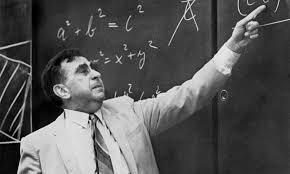
\includegraphics[scale =.44]{edteller}
	 \end{center}
\end{frame}

\begin{frame}{Simulation}{MCMC}
	When the full conditionals are known the Gibbs sampler can be used to get the marginal distirbutions. \\ How it works,
	\begin{itemize}
		\item For R.V.'s $ X, Y $, pick a random $ Y'_0= y_0' $. Then  $ X_j \sim f(x | Y'_j = y_j' ) $
		\item $ Y_{j+1} = f(y |X'_j = x_j') $
		\item Repeat
	\end{itemize}
	The sequence $ Y_0', X_0', , Y_1', X_1', \dots Y_k', X_k' $ converges to the marginal distribution of $ X $ as $ k\rightarrow \infty $
\end{frame}

\begin{frame}{Simulation}{MCMC}
	Doing this with the Linear Regression Model requires full conditionals for $ \beta| \sigma^2, y $ and $ \sigma^2|\beta, y $, which we derived. To start simulation of $ \beta $ and $ \sigma^2 $, 
	\begin{itemize}
		\item Pick an initial value for $ \sigma^{2(0)} $
		\item Calculate $ B_1^{(0)} = [\sigma^{-2(0)} X'X + B_0^{-1}]^{-1}$ and $ \beta_1^{(0)} = B_1^{(0)}[\sigma^{-2(0)}X'y + B_0^{-1}\beta_0 ] $ and generate $ \beta^{0} \sim N_k(\beta_1^{(0)}, B_1^{(0)}) $
		\item Store $ \beta_1^{(0)} $
		\item Generate $ \sigma^{2(1)} \sim IG(\frac{\alpha_1}{2}, \frac{\delta_1^{ (1) }} {2}  )$, $ \delta_1^{(1)} = \delta_0 + (y-X\beta_1^{(0)})'(y-X\beta_1^{(0)}) $
		\item Store $ \sigma^{2(1)} $
		\item Repeat $ N $ times
		\item Burn in $ B $ observations (Delete(Since $ \sigma^{2(0)} $ was not drawn from the distribution the initial observations will not be drawn from the true marginals for a few observations, $ B $, $ 1,000 $ out of 10,000 is frequently done))
	\end{itemize}
\end{frame}

\begin{frame}{Simulation}{MCMC}
	Gibb sampler steps
	\begin{itemize}
		\item Pick an initial value for $ \sigma^{2(0)} $
		\item Calculate $ B_1^{(0)} = [\sigma^{-2(0)} X'X + B_0^{-1}]^{-1}$ and $ \beta_1^{(0)} = B_1^{(0)}[\sigma^{-2(0)}X'y + B_0^{-1}\beta_0 ] $ and generate $ \beta^{0} \sim N_k(\beta_1^{(0)}, B_1^{(0)}) $
		\item Store $ \beta_1^{(0)} $
		\item Generate $ \sigma^{2(1)} \sim IG(\frac{\alpha_1}{2}, \frac{\delta_1^{ (1) }} {2}  )$, $ \delta_1^{(1)} = \delta_0 + (y-X\beta_1^{(0)})'(y-X\beta_1^{(0)}) $
		\item Store $ \sigma^{2(1)} $
		\item Repeat $ N $ times
		\item Burn in $ B $ observations (Delete. Since $ \sigma^{2(0)} $ was not drawn from the distribution the initial observations will not be drawn from the true marginals for a few observations, $ B $, $ 1,000 $ out of 10,000 is frequently done)
	\end{itemize}
\end{frame}

\begin{frame}{MCMCpack}
	Use MCMCpack to do Bayesian regression, \\
	\includegraphics[scale=.5]{headswiss}\\
	breg $<-$ MCMCregress(Fertility $ \sim $ Agriculture + Examination + Education + Catholic + Infant.Mortality, data=swiss)\\
	summary(breg)\\
	See appendix for coding this yourself. 
\end{frame}

\begin{frame}{Results of MCMCregress}
	\begin{center}
	\includegraphics[scale=.5]{bregout}
	\end{center}
\end{frame}

\begin{frame}{Posterior Distributions}
	You won't be able to reproduce this unless you write your own code.
	\centering 
		\includegraphics[width=3cm,, height=3.5cm]{beta1} \hspace{.75cm} \includegraphics[width=3cm,, height=3.5cm]{beta2} \hspace{.75cm} \includegraphics[width=3cm,, height=3.5cm]{beta3}\\
	\centering 
		\includegraphics[width=3cm,, height=3.5cm]{beta4} \hspace{.75cm} \includegraphics[width=3cm,, height=3.5cm]{beta5} \hspace{.75cm} \includegraphics[width=3cm,, height=3.5cm]{sigma}
\end{frame}

\begin{frame}{Results of MCMCregress}
	A confidence interval analog, Bayesian Credible Intervals. This is a probability for the parameter.
	\begin{center}
		\includegraphics[scale=.5]{bquantiles}
	\end{center}
\end{frame}

\begin{frame}{Sensitivity Analysis}
	\begin{itemize}
		\item It is a good idea to include a wide range of prior beliefs to see how sensitive the results are to different priors. Here $ B_0 = 100, 0.001$ on the diagonal as opposed to 1.\\
		\includegraphics[scale=.5]{B0100} \ \includegraphics[scale=.5]{B0001} \\
		Similarly you can play with the other parameters of the Normal and Inverse Gamma. 
	\end{itemize}
\end{frame}

\begin{frame}{Bayes Factor Analysis}
	\begin{itemize}
		\item Consider this a Bayesian Hypothesis test
		\item How likely model $ M_1 $ is the correct model versus model $ M_2 $ versus $ M_3 $, versus $ M_n $
		\item A ratio of one models probability given the data to another
		\item You can do this with MCMCpack using BayesFactor function
	\end{itemize}
\end{frame}

\begin{frame}{Bayes Factor Analysis}{Example}
	brthwt dataset, 3 models:\\
	\includegraphics[scale=.4]{birthwt}
\end{frame}

\begin{frame}{Bayes Factor Analysis}
	\includegraphics[scale=.6]{bayesfactor}
	\begin{itemize}
		\item Showing the results of the log of the division of the probabilities
		\item Compares model $ i $ to model $ j $ where $ i $ is a row $ j $ a column
		\item Model 1 is $ \approx 10^{2.6} $ more likely than model 2.
	\end{itemize}
\end{frame}

\begin{frame}{Bayes Factor Analysis}
	\begin{table}
		\caption{Jeffery's Guidelines}
		\begin{tabular}{ll}
			\hline
			\hline 
			$ \log_{10}(R_{12}) > 2 $ & Decisive support for $ M_1 $ \\
			$ 3/2 < \log_{10}(R_{12}) < 2 $ & Very strong evidence for $ M_1 $ \\
			$ 1 < \log_{10}(R_{12}) < 3/2 $ & Strong evidence for $ M_1 $ \\
			$ 1/2 < \log_{10}(R_{12}) < 1 $ & Substantial evidence for $ M_1 $ \\
			$ 0 < \log_{10}(R_{12}) < 1/2 $ & Weak evidence for $ M_1 $ \\
			\hline
			\hline
		\end{tabular}
	\end{table}
\end{frame}

\begin{frame}{Bayes Factor Analysis}
	Try using package BayesFactor, a break down of every possible model. Show the probability that one model is prefered to a null model.
	\includegraphics[scale=.5]{bayesfactorcode}\\
	\includegraphics[scale=.5]{bayesfactorcompare}
\end{frame}
                                                                                          
\begin{frame}{Bayes Factor Analysis}
	Plot of Bayes Facto,\\
	\includegraphics[scale=.5]{bayesfactorplot}
	Compared to the full model the effect on the Bayes Factor. Blue bars mean dropping that variable \textbf{increases} the Bayes Factor while the converse is true for tan bars. 
\end{frame}

\begin{frame}{Bayes Factor OBR Data}{7 day cruise model}
Below results from $ \log_e $ Bayes Factor MCMC pack function on 5 different models. The full model is to be preferred above the others strong
	\begin{table}
			\scalebox{.8}{
	\begin{tabular}{r|rrrrr}
				                & Full & No inc. & No inc. no egss & No inc., egss, or meta & Null \\
		     \hline 
		Full             		& 0    & 213.3 & 199.6 & 360 & 962 \\
		No inc.           		& -213 & 0.0 & -13.7 & 147 & 749 \\
		 No inc. no egss        & -200 & 13.7 & 0.0 & 161 & 763 \\
		 No inc., egss, or meta & -360 & -146.8 & -160.5 & 0 & 602 \\
		Null & -962 & -749.1 & -762.8 & -602 & 0 \\
		\hline 
	\end{tabular}
}
	\end{table}
\end{frame}

\begin{frame}{Bayes Factor OBR Data}{7 day cruise model}
	Model results for more interesting parameter estimates:\\
	$$\beta = \begin{pmatrix}
		\text{Constant} \\ \text{Shipname} \\ \text{Trade} \\ \text{Nation} \\
		\text{Meta} \\ \text{Loyalty} \\ \text{Income} \\ \text{Net Ticket Revenue} \\ \text{Age} \\
		\text{Rating} \\
	\end{pmatrix} $$
	\[ \text{OBR} = X\beta  + \text{other factors} \] $ X $ is the matrix of data. Shipname-Income are categorical variables.\\ 
	 NTR and Age are continuous.   
\end{frame}

% Data visualization slides begin here
\begin{frame}{Visualizing the Data}
	\includegraphics[scale=.5]{freqcountry}	\includegraphics[scale=.5]{usaheat} 	
\end{frame}

\begin{frame}{Breakdown of Age Groups on Board}
	\includegraphics[scale=.4]{agefreq}
\end{frame}

\begin{frame}{Big Age Group Spenders and Trade and OBR}
	\includegraphics[scale=.3]{bigagespend}
		\includegraphics[scale=.28]{tradespend}
\end{frame}

\begin{frame}{Cruise Length And Spending}
	\includegraphics[scale=.45]{whatif} \ \includegraphics[scale=.5]{shortertrips}
\end{frame}

\begin{frame}{Breakdown of Spending}
	\centering
	\includegraphics[scale=.35]{spendbreakdown}
\end{frame}

\begin{frame}{Shipname Coefficients}
	\begin{table}
		\centering 
		\begin{tabular}{r|r r }
			Shipname & Estimate & Std. Error \\ 
			\hline 
			(Intercept) & 52.7213 & 14.7  \\
			Eurodam & 14.5784 & 2.853 \\
			Koningsdam & 23.0042 & 5.577 \\
			Maasdam & 12.1257 & 3.796  \\
			Nieuw Amsterdam & 10.6858 & 2.654 \\
			Noordam & 7.8171 & 2.244 \\
			Veendam & 14.1696 & 3.648 \\
		\end{tabular}
	\end{table}
	Base category Amsterdam
\end{frame}

% Regerssion coefficients begin here
\begin{frame}{Trade Coefficients}
	\begin{table}
		\centering
		\begin{tabular}{r|rr}
			Trade & Estimate & Std. Error \\ 
			\hline 
			(Intercept) & 52.7213 & 14.7  \\
			Bermuda & -36.0138 & 3.954 \\
			Canada and New England & -24.1643 & 3.490 \\
			Caribbean & -21.3396 & 2.188 \\
			Coastal & -7.6245 & 25.30 \\
			Europe & -12.4955 & 3.463 \\
			Hawaii & -47.3708 & 13.96 \\
			Mexico & -23.5303 & 4.066 \\
			Panama Canal & -42.9484 & 17.60 \\
		\end{tabular}
	\end{table}
	Base category Alaska
\end{frame}

\begin{frame}{Nationality Estimates}
	\begin{table}
		\centering 
	\begin{tabular}{r|rr}
		Nationality & Estimate & Std. Error \\
		\hline 
		(Intercept) & 52.7213 & 14.7  \\
		Canada & -18.6382 & 3.215 \\
		Great Britain & -7.2818 & 4.055 \\
		Netherlands & -19.0230 & 5.417 \\
		United States & -10.0031 & 3.106 \\
		Other & -17.5929 & 4.051 \\
	\end{tabular}
\end{table}
Base category Australia
\end{frame}

\begin{frame}{Income Estimates}
	\begin{table}
		\centering
		\begin{tabular}{r|rr}
			Income & Estimate & Std. Error \\
			\hline
		      (Intercept) & 52.7213 & 14.7  \\			 
			20,000-29,999 & 8.6618 & 4.837 \\
			30,000-49,999 & 9.2675 & 4.191 \\
			50,000-69,999 & 10.9316 & 4.051 \\
			70,000-99,999 & 15.1702 & 3.989 \\
			10,0000-124,999 & 19.0458 & 4.002 \\
			125,000-250,000 & 25.4786 & 3.982 \\
			Over 250,000 & 45.5392 & 4.103 \\
		\end{tabular}
	\end{table}
	Base category under 20,000
\end{frame}

\begin{frame}{Ticket, Age and Rating Estimates}
\begin{table}
	\begin{tabular}{r|rr}
		            & Estimate & Std. Error \\
		            \hline 
		(Intercept) & 52.72 & 14.7 \\
		Net Ticket Rev. & 0.01 & 0.0008 \\
		Age & -0.4206 & 0.039 \\
		Rating & 0.9549 & 0.2734 \\
	\end{tabular}
\end{table}
	
	
\end{frame}

\begin{frame}{Summary}
	\begin{itemize}
		\item Bayesian Analysis is more intuitive
		\item Bayesian point estimates are the means, medians, modes of distributions
		\item Bayesian point estimate standard errors are the standard deviations of posterior distributions
		\item Bayesian interval esitmates (Confidence intervals in Classical statistics) are quantiles of posterior distributions
		\item Bayesian hypothesis testing and model selection can be done using Bayes Factors
		\item Packages that are helpful:
		\begin{itemize}
			\item MCMCpack
			\item BayesFactor
		\end{itemize}
	\end{itemize}
\end{frame}

\begin{frame}{References}
	\begin{itemize}
		\item MCMCpack documentation
		\item \textit{Introduction to Bayesian Econometrics}, \textit{Greenberg}. Available online in pdf
	\end{itemize}
\end{frame}
	
% % % % %
% Appendices 

\begin{frame}{Appendix}{$ \bar{X}'s$ Distribution }
	\begin{block}{Proof}
		By method of M.G.F.'s where
		$$ M_X(\nu) = \mathbb{E}e^{\nu X}  $$ and \[ M_X(\nu) = M_Y(\nu) \iff F_X(u) = F_Y(u) \] 
		The M.G.F. uniquely identifies the distribution of $ X $. It is known the M.G.F. of $ X \sim N(\mu,\sigma) $ is $ e^{\mu\nu +  \sigma^2\frac{\nu^2}{2}} $. The M.G.F. of $ \bar{X} $ is:
		\[ M_{\bar{X}} = M_{\frac{1}{T}(X_1 + X_2 + \dots + X_T)}(\nu) = M_{(X_1 + X_2 + \dots + X_T)}(\frac{\nu}{T}) \]
		\[ = M_{X_1}(\frac{\nu}{T}) \times  M_{X_2}(\frac{\nu}{T})\times\cdots\times M_{X_T}(\frac{\nu}{T}) \]
	\end{block}
\end{frame}

\begin{frame}{Appendix}{$ \bar{X} $'s distribution}
	\begin{block}{Cont'd Proof}
		Therefore, 
		\[ M_{X_2}(\frac{\nu}{T})\times\cdots\times M_{X_T}(\frac{\nu}{T}) \]
		\[ =  \prod_{i=1}^{T} e^{\mu \frac{\nu}{T} +  \sigma^2 (\frac{\nu}{T})^2 \frac{1}{2}} = e^{T(\mu \frac{\nu}{T} +  \sigma^2 (\frac{\nu}{T})^2 \frac{1}{2})}\]
		\[ =  e^{\mu\nu +  \frac{\sigma^2}{T} \frac{\nu^2}{2}} \]
		Which is a normal distribution $ N(\mu, \frac{\sigma^2}{T}).  $
		Therefore, the \textbf{sample average} has a Normal distribution. 
	\end{block}
\end{frame}

\begin{frame}{Appendix}{Application-Normal Linear Regression Model}
	\[ \pi(\beta, \sigma^2 | x) = \frac{  \mathscr{L}(\beta, \sigma^2;x) N_K(\beta_0, \Sigma) IG(\frac{ \alpha_0 }{2}, \frac{ \delta_0 }{2}  ) }{ f(x) } \]
	or, 
	\[ \pi(\beta, \sigma^2 | x) \propto  \mathscr{L}(\beta, \sigma^2;x) N_K(\beta_0, B_0) IG(\frac{ \alpha_0 }{2}, \frac{ \delta_0 }{2}  )  \]
	Inverse-Gamma probability density function:\\
	If $ x \sim \Gamma(\alpha, \beta) $ with pdf and $ Y = 1/X $ then,
	\begin{align*}
	f(x) = &  \frac{1}{ \Gamma(\alpha)\beta^{\alpha} } x^{\alpha-1} e^{-x/\beta}, \  x > 0 \\
	f(y) = & \frac{ (1/\beta)^{\alpha} }{\Gamma(\alpha) } y^{-(\alpha + 1) } e^{-\frac{ (1/\beta) }{ y }}, \ y>0 
	\end{align*}
\end{frame}

\begin{frame}{Appendix}{Application-Normal Linear Regression Model}
	Using matrix notation ($ \sum_{i=1}^{T} (x_i - \mu)^2 = (X -\mu)'(X-\mu) ) $
	
	\[\pi(\beta, \sigma^2 | x) \propto  (2\pi\sigma^2)^{-T/2} \exp\Big[ -\frac{1}{2\sigma^2}(y-X\beta)'(y-X\beta) \Big] \times \]
	\[ (2\pi\sigma^2)^{-(K/2)} \exp\Big[ -\frac{1}{2\sigma^2}(\beta - \beta_0)'B_0^{-1}(\beta - \beta_0) \Big] \times  \]
	\[ \frac{(\frac{1}{\delta_0/2} )^{\alpha_0/2}}{\Gamma(\alpha_0/2)}  \Big(\frac{1}{\sigma^2}\Big)^{\frac{\alpha_0}{2} + 1} \exp\Big[ -\frac{\delta_0}{2\sigma^2} \Big] \]
	We can proportion out everything that does not involve at $ \beta $
\end{frame}

\begin{frame}{Appendix}{Application-Normal Linear Regression Model}
	Simplified:
	\[  \pi(\beta, \sigma^2 | x) \propto \Big(\frac{1}{\sigma^2} \Big)^{  \frac{(T + \alpha_0)}{2} + 1 } \times
	\Big(\frac{1}{\sigma^2} \Big)^{  K/2 } \times \]
	\[ \exp\Big[-\frac{1}{2\sigma^2}\Big((y-X\beta)'(y-X\beta) + (\beta - \beta_0)'B_0^{-1}(\beta - \beta_0) + \delta_0\Big)\Big] \]
	\begin{itemize}
		\item Next step is expanding the terms inside the big parentheses 
	\end{itemize} 
\end{frame}

\begin{frame}{Appendix}{Application-Normal Linear Regression Model}
	\framesubtitle{All of the algebra details...}
	Considering only the elements in the (...):
	\[ y'y - 2y'X\beta + \beta'X'X\beta + \beta'B_0^{-1} \beta - 2\beta'B_0^{-1}\beta_0 + \beta_0B_0^{-1}\beta_0 + \delta_0 \]
	We will need to factor what is below, 
	\[ (y'y + \beta_0'\Bzero \beta_0 + \delta_0) + (\beta'\Bzero \beta  -2y'X\beta -2\beta'\Bzero\beta_0 + \beta'X'X\beta)   \]
	Factor out the $ -2\beta' $, factor out the $ \beta $'s, 
	\[ (y'y + \beta_0'\Bzero \beta_0 + \delta_0) +  (\beta'(\Bzero + X'X)\beta  -2\beta'(X'y + \Bzero\beta_0)) \]
	Trick: complete the square,
	\begin{itemize}
		\item Consider a multivariate normal with exponent that has an exponent in a quadratic form,
		\[ (x-\mu)\Sigma^{-1}(x-\mu) \]
	\end{itemize}
\end{frame}

\begin{frame}{Appendix}{Application-Normal Linear Regression Model}
	\framesubtitle{All of the algebra details...}
	\begin{itemize}
		\item Consider a multivariate normal with exponent that has an exponent in a quadratic form,
		\[ (x-\mu)\Sigma^{-1}(x-\mu) \]
		\item Multiplying out gives,
		\[ x'\Sigma^{-1}x - 2x'\Sigma^{-1}\mu + \mu'\Sigma^{-1}\mu \]
		\item Clearly $ \mu = \Sigma \Sigma^{-1} \mu $
		\item We can use this trick to refactor our expression, we know we want a MVN random variable, therefore we just need to multiply by the correct expression and add and subtract 1 to fix it
	\end{itemize}
\end{frame}

\begin{frame}{Appendix}
	\framesubtitle{All of the algebra details...}
	Rename some of our variables for ease, 
	\begin{itemize}
		\item $ B_1 = (X'X + \Bzero)^{-1} $ (like $ \Sigma $)
		\item $ \beta_1 =  B_1(X'y + \Bzero\beta_0) $ (like $ \Sigma^{-1}\mu $)
		\item Therefore we can rewrite our expression on the previous slide as
		\[ \beta'B_1^{-1} \beta - 2\beta' B_1^{-1}\beta_1 + \beta_1'B_1^{-1}\beta_1 - \beta_1'B_1^{-1}\beta_1 \]
		\item Notice that  $ \beta_1'B_1^{-1}\beta_1 = ( (X'X + \Bzero)^{-1} (X'y + \Bzero\beta_0) )' (X'X + \Bzero) (X'X + \Bzero)^{-1} (X'y + \Bzero\beta_0)  $
		\item No terms involve $ \beta $, it can be factored out
	\end{itemize}
\end{frame}

\begin{frame}{Appendix}
	\framesubtitle{All of the algebra details...}
	Therefore,
	\[ (y'y + \beta_0'\Bzero \beta_0 + \delta_0) +  (\beta'(\Bzero + X'X)\beta  -2\beta'(X'y + \Bzero\beta_0)) = \]
	\[ (y'y + \beta_0'\Bzero \beta_0 + \delta_0 - \beta_1 B_1^{-1}\beta_1) + (\beta-\beta_1)'B_1^{-1}(\beta-\beta_1) \]
	Redefine $ \delta $ in the inverse gamma, $ \delta_1 =  (y'y + \beta_0'\Bzero \beta_0 + \delta_0 - \beta_1 B_1^{-1}\beta_1) $ and redefine $ \alpha_1 = T + \alpha_0 $ \\
	We can rewrite the entire equation as,
	\[ \pi(\beta,\sigma^2|y) \propto  \Big(\frac{1}{\sigma^2} \Big)^{  \frac{(\alpha_1)}{2} + 1 } \times \exp\Big[ -\frac{\delta_1}{2\sigma^2}\Big] \times\] 
	\[\Big(\frac{1}{\sigma^2} \Big)^{  K/2 } \times \exp\Big[-\frac{1}{2\sigma^2}\Big((\beta-\beta_1)'B_1^{-1}(\beta-\beta_1)  \Big)\Big] \] 
\end{frame}

\begin{frame}{Appendix}{Normal-Linear Regression}
	Assuming unequal variances conditional for $ \beta $, $ \pi(\beta|\sigma^{2}, y) $, 
	\[\pi(\beta, \sigma^2 | x) \propto  (2\pi\sigma^2)^{-T/2} \exp\Big[ -\frac{1}{2\sigma^2}(y-X\beta)'(y-X\beta) \Big] \times \]
	\[ (2\pi\mu^2)^{-(K/2)} \exp\Big[ -\frac{1}{2\mu^2}(\beta - \beta_0)'B_0^{-1}(\beta - \beta_0) \Big] \times  \]
	\[ \frac{(\frac{1}{\delta_0/2} )^{\alpha_0/2}}{\Gamma(\alpha_0/2)}  \Big(\frac{1}{\sigma^2}\Big)^{\frac{\alpha_0}{2} + 1} \exp\Big[ -\frac{\delta_0}{2\sigma^2} \Big] \]
\end{frame}

\begin{frame}{Appendix}{Normal-Linear Regression}
	Proportion out the $ \mu $
	\[	\pi(\beta, \sigma^2 | x) \propto (\sigma^2)^{-(\frac{\alpha_0 + n}{2} + 1)} \exp\Big[-\frac{\delta_0}{2\sigma^2}\Big] \times    \]
	\[ \exp\Big[ -\frac{1}{2}(\sigma^{-2}(y-X\beta)'(y-X\beta) + (\beta-\beta_0)'\Bzero(\beta - \beta_0))   \Big] \]
	Simplying the expression and following largely the same steps from before (this time proportion out everything without a $ \beta $),
	\[ \beta'(X'X\sigma^{-2} + B^{-1})\beta - 2\beta'(X'y\sigma^{-2} - B_0^{-1}\beta_0 )  \]
\end{frame}

\begin{frame}{Appendix}{Normal-Linear Regression}
	Now complete the square, 
	\begin{description}
		\item $ B_1 = (X'X\sigma^{-2}+B_0^{-1})^{-1} $
		\item $ \beta_1 = B_1(X'y\sigma^{-2} - B_0^{-1}\beta_0) $
	\end{description}
	Therefore the conditional for $ \beta $, $ \pi(\beta|\sigma^{2}, y) $ is $ MVN(\beta_1, B_1)  $. \\
	\textbf{Note the conditional distribution is not the marginal distribution as we were able to obtain with equal variances. Additional work must be done to obtain it.}
\end{frame}

\begin{frame}{Appendix}{Normal-Linear Regression}
	For the variance proportion out anything without a $ \sigma^2 $. 
	\[ \Big(\frac{1}{\sigma^2}\Big)^{\frac{\alpha_1}{2} + 1} \exp\Big[ -\frac{\delta_1}{2\sigma^2} \Big] \]
	\begin{description}
		\item $ \alpha_1 = \alpha_0 + T$
		\item $ \delta_1 = \delta_0 + (y-X\beta)'(y-X\beta) $
	\end{description}
	$ \sigma^2|\beta, y $ has $ IG(\frac{\alpha_1}{2}, \frac{\delta_1}{2}) $
\end{frame}

\begin{frame}{Appendix}{Actually Doing This In Code}
	\begin{description}
		\item	\includegraphics[scale=.5]{swissdata}
		\item Standardized fertility measure and socio-economic indicators for each of 47 French-speaking provinces of Switzerland at about 1888. \\
		\includegraphics[scale = .35]{headswiss}
		\item 
	\end{description}
\end{frame}

\begin{frame}{Appendix}{Actually Doing This In Code}
	What if we wanted the marginal effects of one of the variables on fertility? 
	\begin{description}
		\item \includegraphics[scale = .5]{collectdata}
		\item $ y = (y_1, y_2, \dots  y_47)' $ observations on fertility. $ X = (
		Agr \ Exam  \ Educ  \ Cath \ InfM ) $, where each variable is a column vector of 47 elements. 
		\item $ \beta = (\beta_{1}, \beta_2, \dots, \beta_5) $
		\item $ y = X\beta + u $
	\end{description}
\end{frame}

\begin{frame}{Appendix}{Tuning Parameters}
	Specify priors, \\
	\begin{center}
		\includegraphics[scale=.5]{priors}
	\end{center}
	\begin{itemize}
		\item Mean of IG = $ \frac{\beta}{\alpha - 1} $, Variance =$ \frac{\beta^2}{(\alpha-1)^2(\alpha-2)}  $, what is a reasonable variance for $ u $?
		\item The Min is 35, the Max is 92.5, most of the data will be between there, a standard deviation of about 16 is reasonable for y
		\item The variance of $ u $ will be less with our covariates, say 10. 
		\item Therefore $ \delta_0 = 20 $, $ \alpha_0 = 6 $ to reflect uncertainty. 
		\item You can specify the $ B_0 $ matrix using the Hessian of the maximum likelihood estimators. For now let it be the identity matrix. 
	\end{itemize}
\end{frame}

\begin{frame}{Appendix}{Tuning Parameters}
	\begin{itemize}
		\item $ \beta_0 $ can be set to be $ 0 $ or the estimates from maximum likelihood or from a regression. 
		\item \includegraphics[scale=.4]{gibb}
	\end{itemize}
\end{frame}

\begin{frame}{Appendix}{Means Of Posterior Distributions}
\begin{table}
		\scalebox{.55}{
			\begin{tabular}{r|ccccccc}
				& Constant & $ \beta_1 $ & $ \beta_2 $ & $ \beta_3 $ & $ \beta_4 $ & $ \beta_5 $ & $ \sigma^2 $/ Residual variance \\
				\hline 
				Posterior Mean $ \alpha_0 = 6, \delta_0 = 20 $ & 66.915 & -0.172 & -0.258 &  -0.871 &  0.104 &  1.077 & 47.151  \\
				Posterior Mean $ \alpha_0 = 12, \delta_0 = 20 $ & 66.915 & -0.172 & -0.258 &  -0.871 &  0.104 &  1.077 & 41.571  \\
				Posterior Mean $ \alpha_0 = 18, \delta_0 = 20 $ & 66.893 & -0.172 & -0.257 &  -0.871 &  0.104 &  1.077 &  37.103  \\
				Posterior Mean $ \alpha_0 = 18, \delta_0 = 1 $ & 66.868 & -0.172 & -0.256 &  -0.871 &  0.104 &  1.078 &  36.871  \\
				Linear Regression Estimates & 66.915 & -0.172 &  -0.258 & -0.871 &  0.104 &  1.077 & 45.7618 \\
				MCMCregress & 67.0208 & -0.1724 & -0.2586 & -0.8721 & 0.1040 & 1.0737 & 54.0498 \\
				\hline 
			\end{tabular}
		}
		\caption{Sensitivity Analysis and comparison}
	\end{table}
\end{frame}

\begin{frame}{Appendix}{Bayesian Credible Intervals}
	\begin{table}
		Confindence intervals are straightforward, they are the quantiles of the posterior. \\
		\scalebox{.55}{
			\begin{tabular}{r|ccccccc}
				& constant & Agriculture & Examination &  Education&   Catholic & Infant.Mortality &   $ \sigma^2 $ \\
				\hline 
				Post. Mean &67.03231 &-0.17313848 & -0.2591934 &-0.8720746 & 0.1040975   &     1.0749401 & 47.26015 \\
				95\%        &83.98964 &-0.06113534 &  0.1423363 & -0.5779736 &0.1591103   &     1.6750191 & 65.96488 \\
				5\%        &50.16641 &-0.28473593 & -0.6620177 &-1.1652054 & 0.0489915    &    0.4777965 &33.25929 \\
				\hline 
			\end{tabular}
		}
	\end{table}
\end{frame}

\end{document}
